\documentclass[12pt]{article}
\usepackage[margin=1in]{geometry}
\usepackage{graphicx}
\usepackage{booktabs}
\usepackage{amsmath}
\usepackage{amssymb}
\usepackage{float}
\usepackage{caption}
\usepackage{setspace}
\usepackage[most]{tcolorbox}
\captionsetup{font=small, labelfont=bf, skip=6pt}
\onehalfspacing

\newtcolorbox{explain}{%
  colback=black!3,
  colframe=black!25,
  boxrule=0.5pt,
  arc=1pt,
  left=8pt,
  right=8pt,
  top=5pt,
  bottom=5pt,
  before skip=6pt,
  after skip=12pt,
  fontupper=\normalsize
}

\title{LSTM\\[0.2em]
\large Bitcoin realized volatility}
\author{Volatility forecasting project}
\date{30 September 2026}

\begin{document}
\maketitle

\noindent
Separate LSTM results under frozen Protocol~B.
Script: \texttt{models/run\_lstm.py}.
Classical baselines stay in \texttt{baselines\_report.pdf}.

\section{Setup}
\begin{itemize}
  \item Target: $y_t=\log\mathrm{RV}_{t+1}$ (same as baselines).
  \item Forecast: HAR plus an LSTM residual,
  \[
  \hat y_t=\widehat{\mathrm{HAR}}_t+w\cdot f_{\mathrm{LSTM}}(x_{t-L+1:t}).
  \]
  Channels in the window: $\log\mathrm{RV}$, its 7-day and 22-day means, $R_t^2$, and volume $z$.
  \item $w=0$ is pure HAR. $w$ is chosen on val together with the other hyperparameters.
  \item Scaler: per-channel mean/std fit on the fitting sample only
    (train while tuning; train+val on final refit).
  \item Optimizer: Adam. Loss: MSE on the residual.
  \item Val (2022--2023): grid + early stopping. Test never used for tuning.
\end{itemize}

\section{Hyperparameter grid}
Small chronological search (not $k$-fold CV):
\[
L\in\{22,60\},\quad
h=64,\quad
\mathrm{depth}\in\{1,2\},\quad
\mathrm{dropout}\in\{0.1,0.2\},\quad
\mathrm{LR}\in\{10^{-3},3\cdot10^{-4}\}.
\]
16 configs. Each trained on train with early stopping on val forecast RMSE
(patience 10, max 80 epochs). Best config then refit on train+val for the chosen epoch budget, with $w$ frozen.

\begin{figure}[H]
\centering
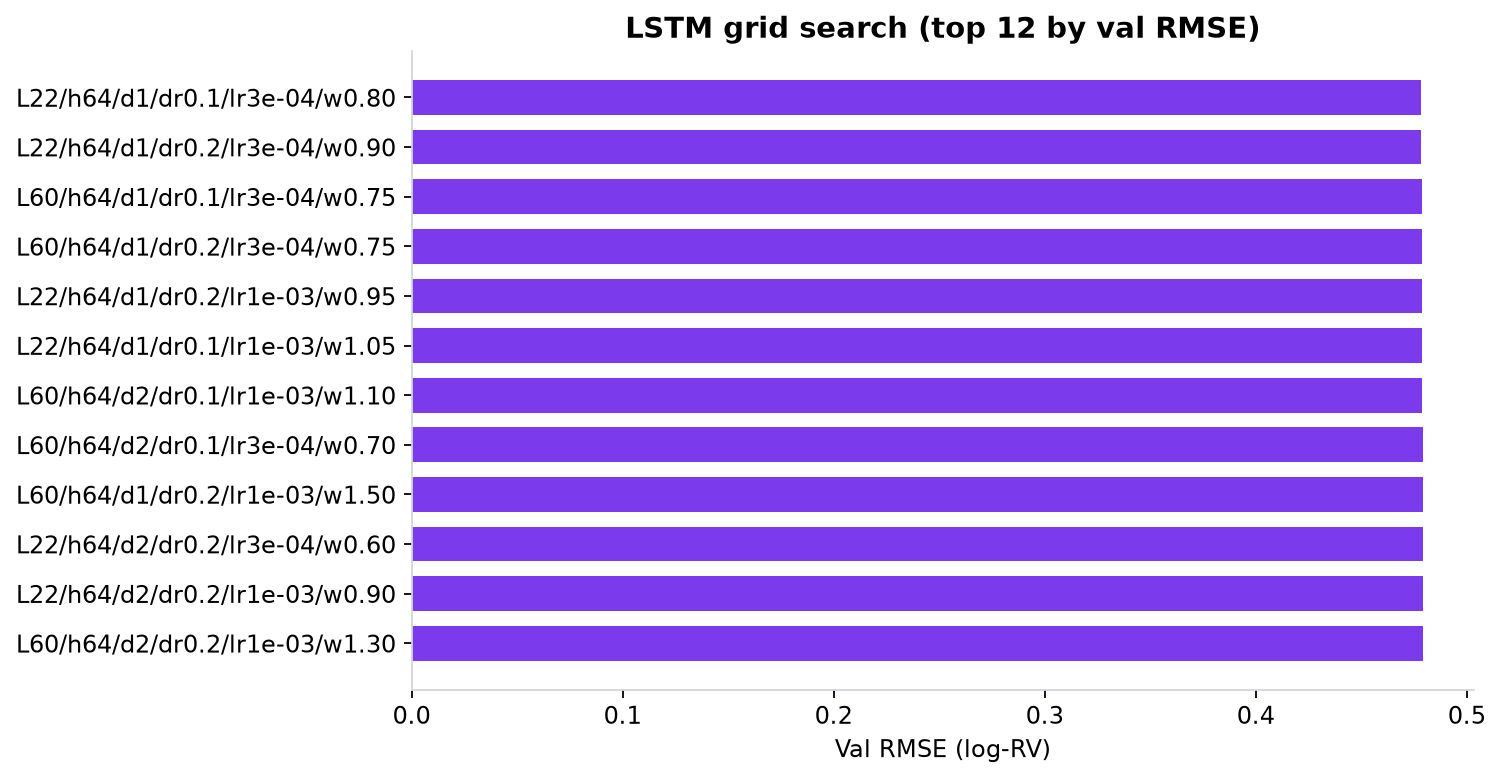
\includegraphics[width=\textwidth]{figures/lstm_val_grid.png}
\caption{Top 12 grid configs by validation RMSE.}
\end{figure}

\begin{figure}[H]
\centering
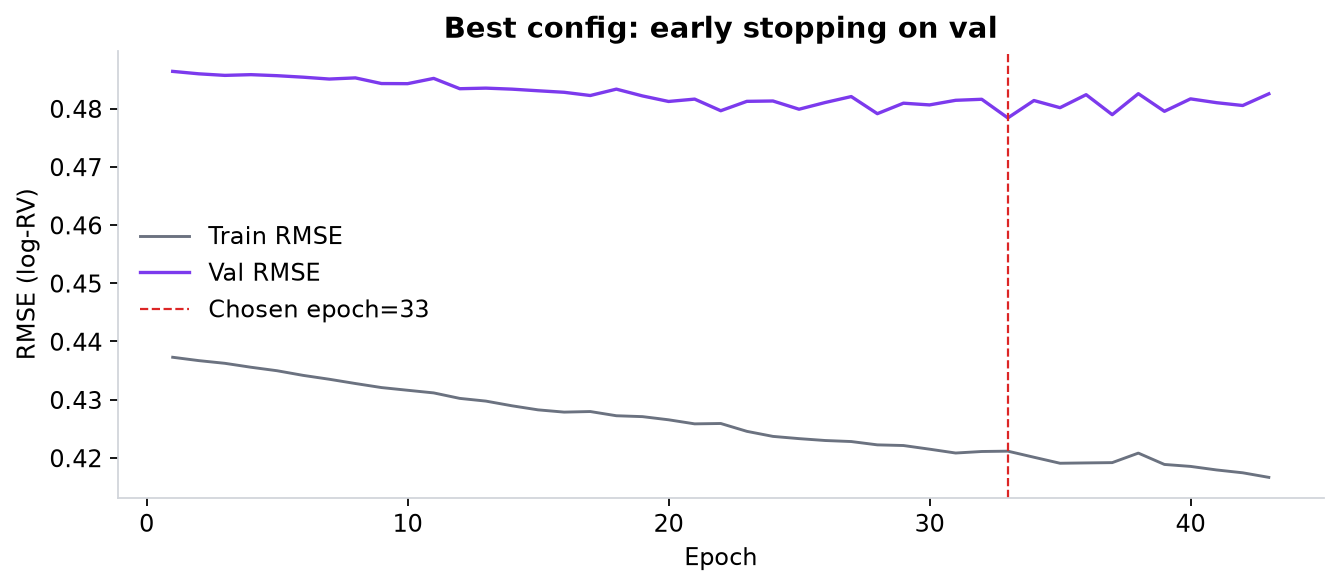
\includegraphics[width=0.95\textwidth]{figures/lstm_learning_curve.png}
\caption{Train vs val RMSE for the winning config; red line = chosen epoch.}
\end{figure}

\section{Selected model}
\begin{table}[H]
\centering
\begin{tabular}{lr}
\toprule
Setting & Value \\
\midrule
$L$ (lookback) & 22 \\
Hidden size & 64 \\
Depth & 1 \\
Dropout & 0.1 \\
Learning rate & $3\times10^{-4}$ (Adam) \\
Residual weight $w$ & 0.80 \\
Best val epoch & 33 \\
Val RMSE & 0.478 \\
\bottomrule
\end{tabular}
\caption{Winning hyperparameters from the val grid.}
\end{table}
\begin{explain}
Refit on train+val for 33 epochs with frozen settings (including $w$), then score test once.
\end{explain}

\section{Test results}
$n=999$ (2024-01-01 through 2026-09-25). Naive and HAR shown for context on the same rows.

\begin{table}[H]
\centering
\begin{tabular}{lrrr}
\toprule
Model & RMSE & MAE & QLIKE \\
\midrule
Naive & 0.560 & 0.444 & 0.161 \\
HAR & 0.458 & 0.354 & 0.101 \\
\textbf{LSTM} & \textbf{0.448} & \textbf{0.349} & \textbf{0.099} \\
\bottomrule
\end{tabular}
\caption{Test metrics on $\log\mathrm{RV}$ (RMSE/MAE) and RV (QLIKE).}
\end{table}

\begin{figure}[H]
\centering
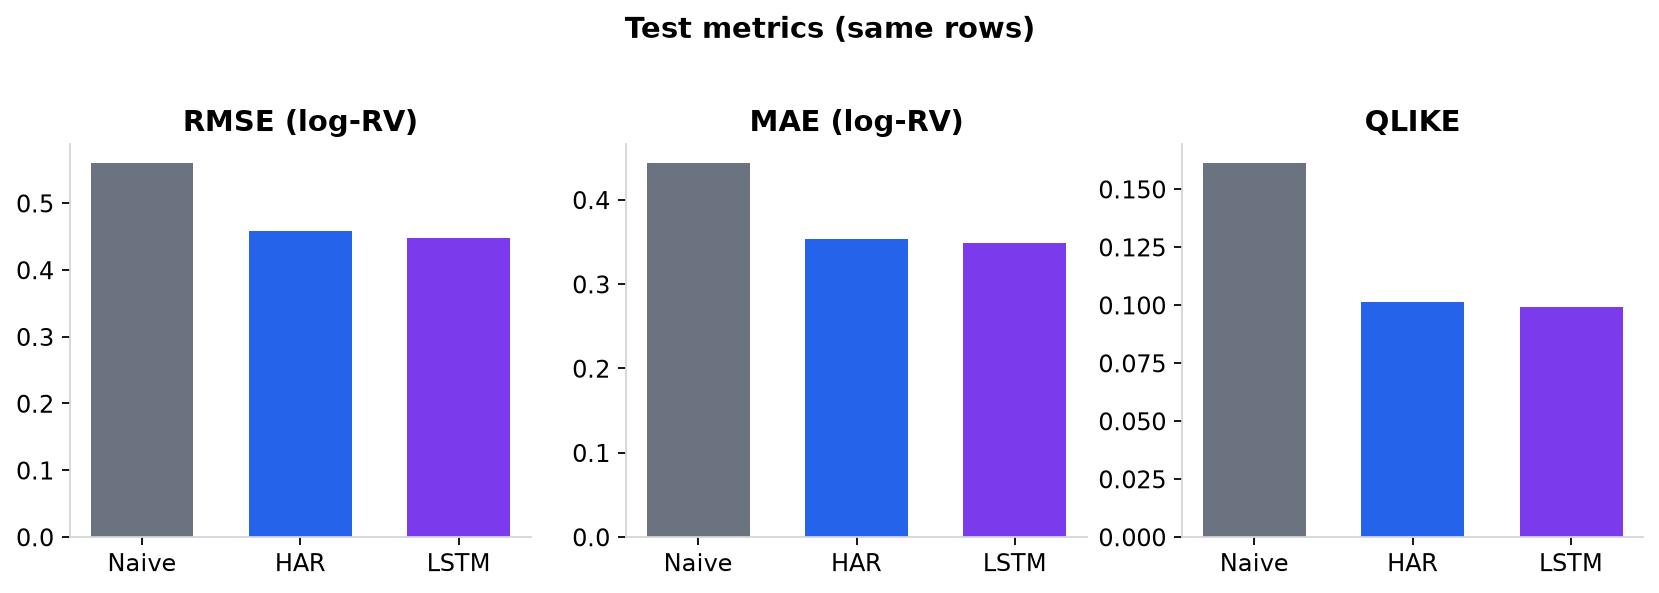
\includegraphics[width=\textwidth]{figures/lstm_test_metrics.png}
\caption{Test RMSE / MAE / QLIKE: Naive, HAR, LSTM.}
\end{figure}

\begin{explain}
On the test set the HAR--LSTM forecast improves on HAR and Naive in RMSE, MAE, and QLIKE.
The gain over HAR is modest, consistent with a persistent realized-volatility target.
\end{explain}

\begin{figure}[H]
\centering
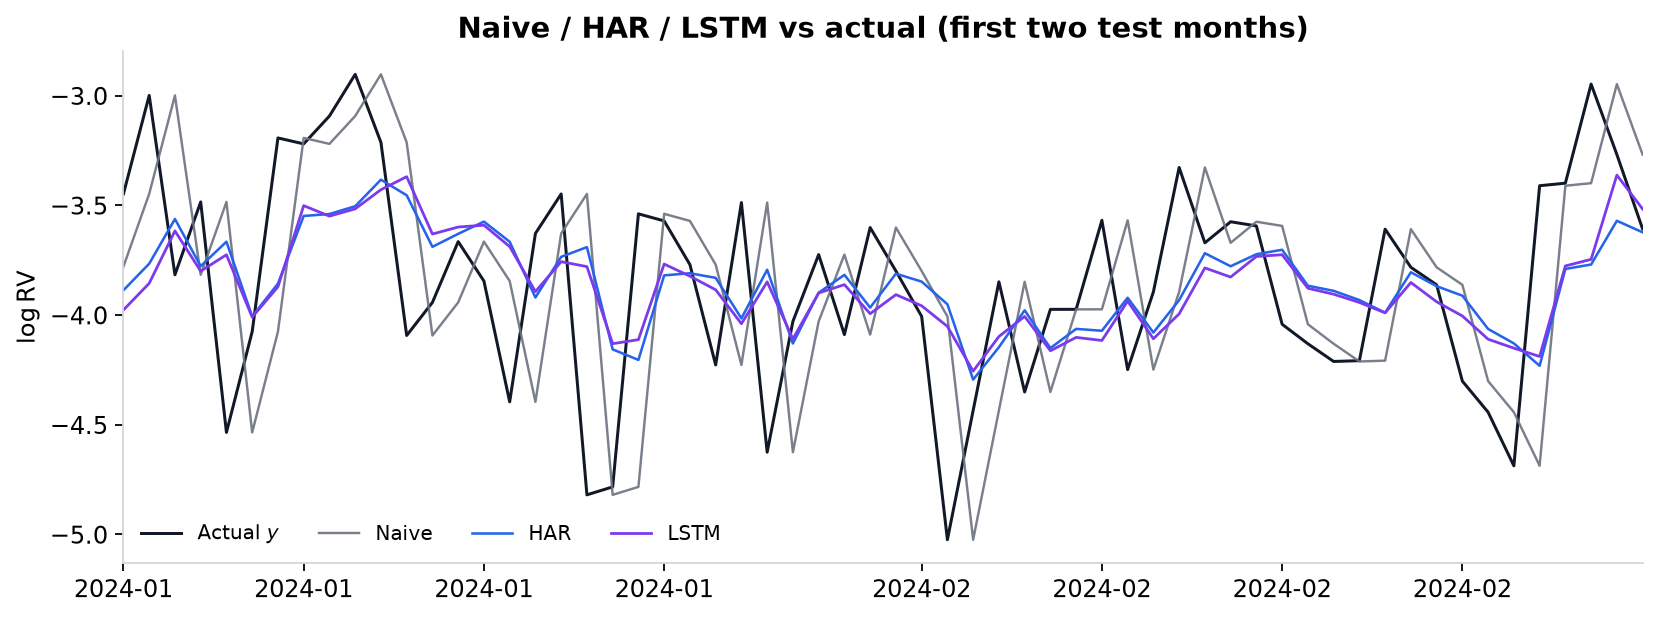
\includegraphics[width=\textwidth]{figures/lstm_test_paths_2mo.png}
\caption{Naive, HAR, and LSTM vs actual (first two test months).}
\end{figure}
\begin{figure}[H]
\centering
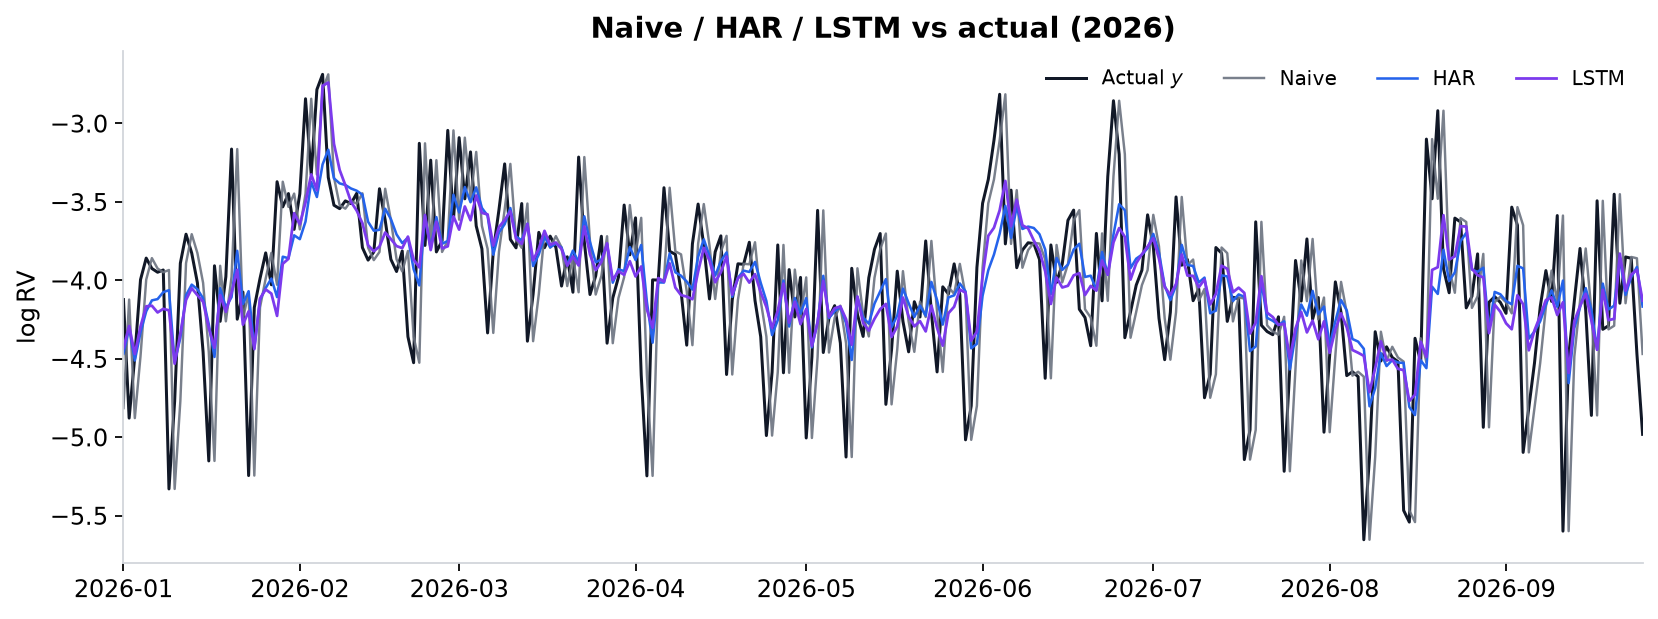
\includegraphics[width=\textwidth]{figures/lstm_test_paths_2026.png}
\caption{Naive, HAR, and LSTM vs actual (calendar 2026).}
\end{figure}

\section{Takeaway}
\begin{explain}
Hyperparameters and the residual weight were selected on the validation window only.
The reported test scores are from a single evaluation after the train+val refit.
\end{explain}

\end{document}
